\subsection{Interfaz gráfica de usuario}
	\label{sec:AGG_GUI}
		
	Una vez el bitstream generado es cargado en la FPGA, se puede visualizar la interfaz gráfica generada por el AGG. El AGG genera la interfaz gráfica de usuario utilizando la información provista por el RNA. Adicionalmente, el AGG gestiona la comunicación entre la FPGA y la interfaz gráfica. Para esto, el AGG actualiza las tramas a enviar a la FPGA y analiza las tramas de respuesta de la FPGA. Las tramas recibidas por el AGG son reinyectadas a la FPGA hasta que exista una convergencia entre las entradas y salidas de la FPGA, tal cómo fue explicado en la Sección \ref{sec:AGG}.
		
	En la Figura \ref{fig:EJ1_AGG} se ilustra la ventana de la interfaz gráfica para el ejemplo 1. El usuario puede realizar zoom en cualquier zona de la interfaz gráfica utilizando la rueda del mouse y desplazarse utilizando el click izquierdo mientras se presiona la tecla shift. Estas funcionalidades son de utilidad en topologías de gran tamaño o, en el caso de este ejemplo, para hacer foco en algunas zonas de mayor interés para el usuario.
	
	\begin{figure}[H]
		\centering
		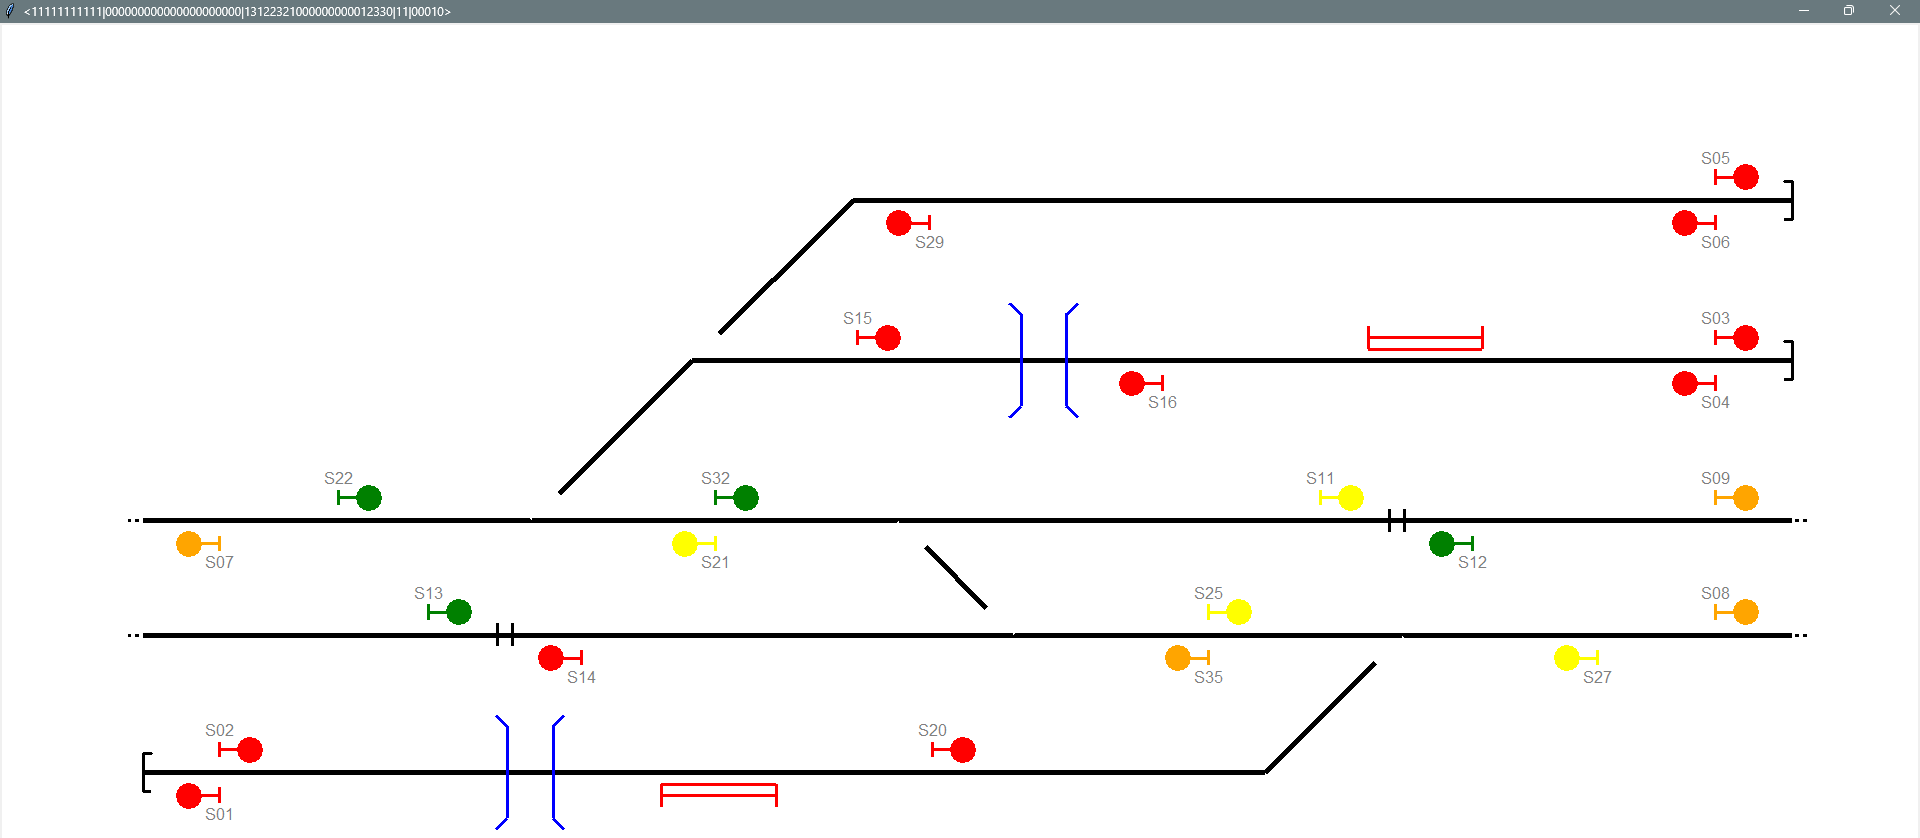
\includegraphics[origin = c, width=1\textwidth]{resultados-obtenidos/ejemplo1/images/AGG_S32_YES}
		\centering\caption{Interfaz gráfica del ejemplo 1.}
		\label{fig:EJ1_AGG}
	\end{figure}
	
	A modo de ejemplo, para demostrar las funcionalidades del sistema de enclavamientos implementado, si se selecciona el \textit{netElement} ne22, el AGG reportará el cambio de estado a la FPGA y esa sección cambiará su color a rojo. En pocos segundos la FPGA responderá con el nuevo estado del señalamiento, ilustrado en la Figura \ref{fig:EJ1_AGG_S32_OCCUPIED}. La señal S32 cambiará a rojo para impedir que una formación ingrese a la sección ocupada y la señal S22 cambiará a naranja, aplicando el doble recubrimiento (ver Sección \ref{sec:function_5}). El resto del señalamiento no se modificará ya que la situación local de cada señal no se modificó. Por ejemplo, la implementación del sistema en la FPGA hará que la señal S29 siga en color rojo, para evitar un descarrilamiento, porque el trayecto que tiene a continuación se encuentra desconectado del resto de la red, porque el cambio de vías Sw04 se encuentra en posición reversa.
	
	\begin{figure}[H]
		\centering
		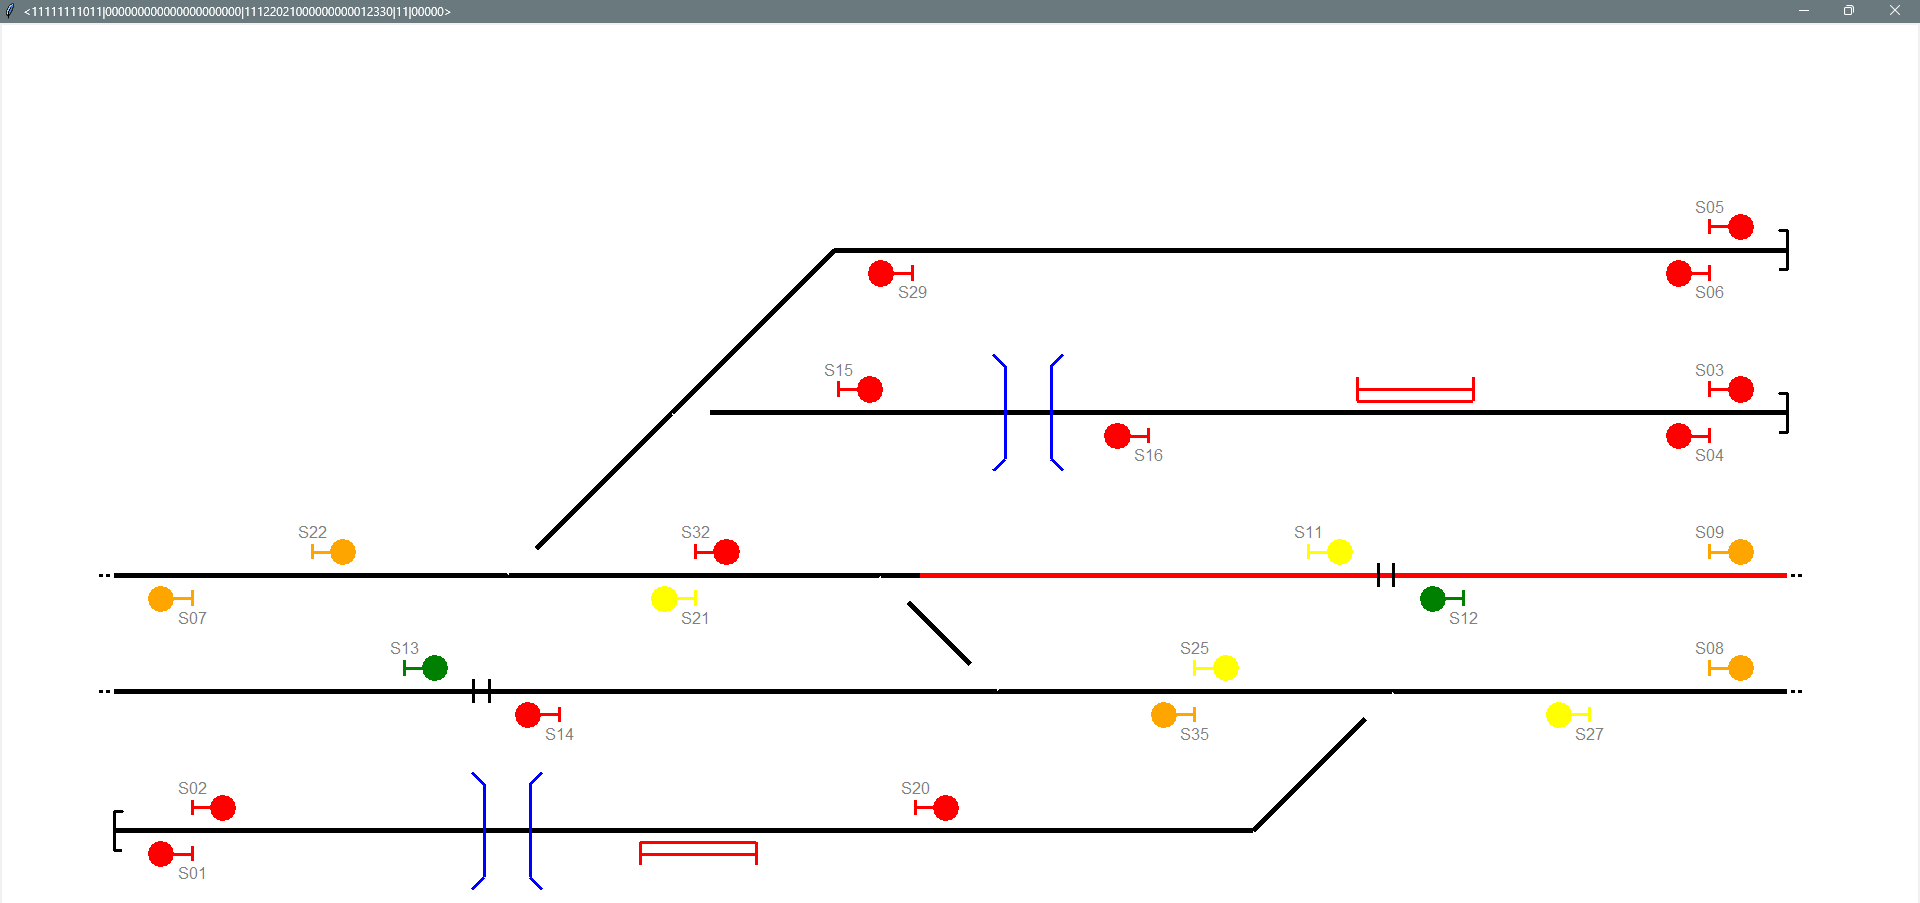
\includegraphics[origin = c, width=1\textwidth]{resultados-obtenidos/ejemplo1/images/AGG_S32_OCCUPIED}
		\centering\caption{Nuevo señalamiento con ne22 ocupado.}
		\label{fig:EJ1_AGG_S32_OCCUPIED}
	\end{figure}

	Si en lugar de ocupar ne22 se selecciona el cambio Sw12, para modificar su posición a reversa, se obtiene la Figura \ref{fig:EJ1_AGG_SW12_REVERSE}. En este caso, el sistema de enclavamiento cambia ambas señales S32 y S22 a rojo, para evitar un descarrilamiento producto de que el cambio Sw12 se encuentra en posición reversa pero el cambio Sw13 aún se encuentra en posición normal.		
	
	\begin{figure}[H]
		\centering
		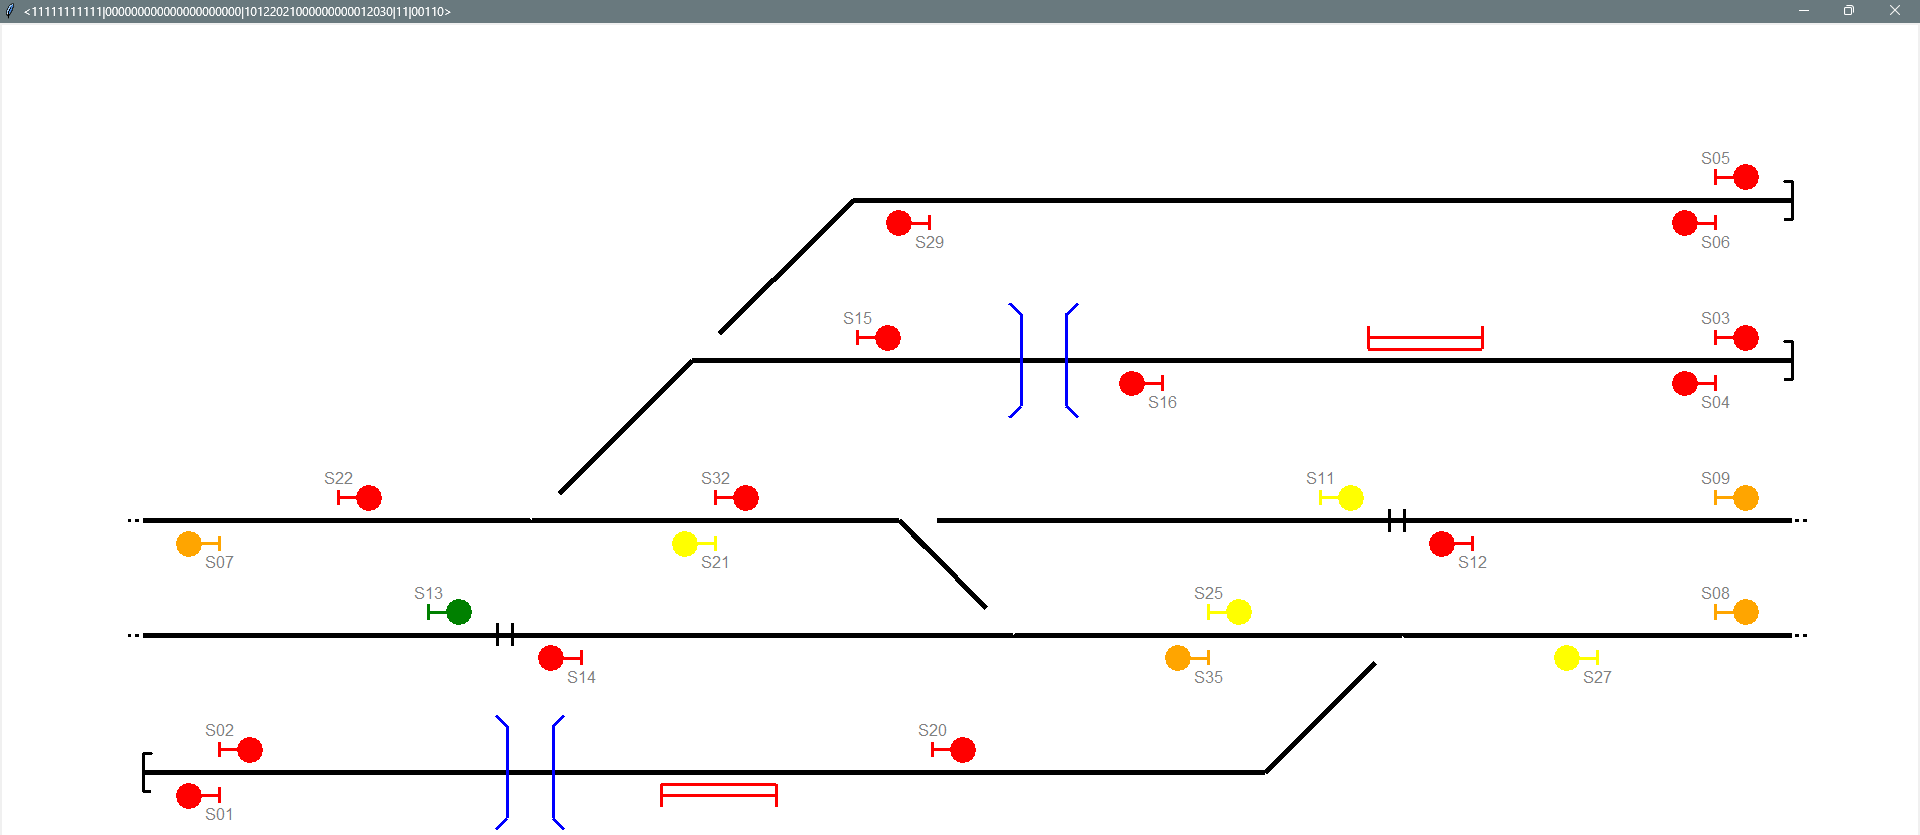
\includegraphics[origin = c, width=1\textwidth]{resultados-obtenidos/ejemplo1/images/AGG_S32_NO}
		\centering\caption{Nuevo señalamiento con Sw12 en reversa.}
		\label{fig:EJ1_AGG_SW12_REVERSE}
	\end{figure}
	
	Tal cómo fue explicado en la Sección \ref{sec:AGG}, las rutas pueden ser solicitadas o canceladas desde la interfaz gráfica seleccionando el nombre de las señales. Cuando una señal es seleccionada, su nombre cambia a color verde y todas las señales candidatas a ser señal de finalización de ruta cambiarán su nombre a rojo. El nombre de las señales restantes cambia a color gris. Sí se vuelve a seleccionar la señal de inicio, el AGG envía a la FPGA un comando de ruta cancelada para todas las rutas que inician con esa señal. Sí se selecciona una de las rutas candidatas a ser señal de finalización de la ruta, el AGG envía la solicitud de esa ruta a la FPGA.
	
	La Figura \ref{fig:EJ1_AGG_R13}	ilustra el caso de solicitud y aprobación de la ruta R13, para lo cual el usuario seleccionó la señal S22 y luego la señal S05. Debido a que ninguna otra ruta se encontraba operativa, la FPGA puede enviar el comando de reserva y enclavamiento de las vías y la infraestructura, tal fue explicado en la Sección \ref{sec:function_2}. El cambio de vías Sw04 pasa a posición reversa, el cambio de vías Sw07 pasa a posición normal y todo el trayecto queda enclavado, tal cómo fue explicado en la Sección \ref{sec:function_1}, ilustrado en color gris. Además, la señal S22, que da inicio a la ruta, pasa a color verde y la señal S05 de finalización de ruta pasa a color rojo. Todas las señales opuestas a la ruta R13, tales cómo C29, pasan a color rojo. 
	
	\begin{figure}[H]
		\centering
		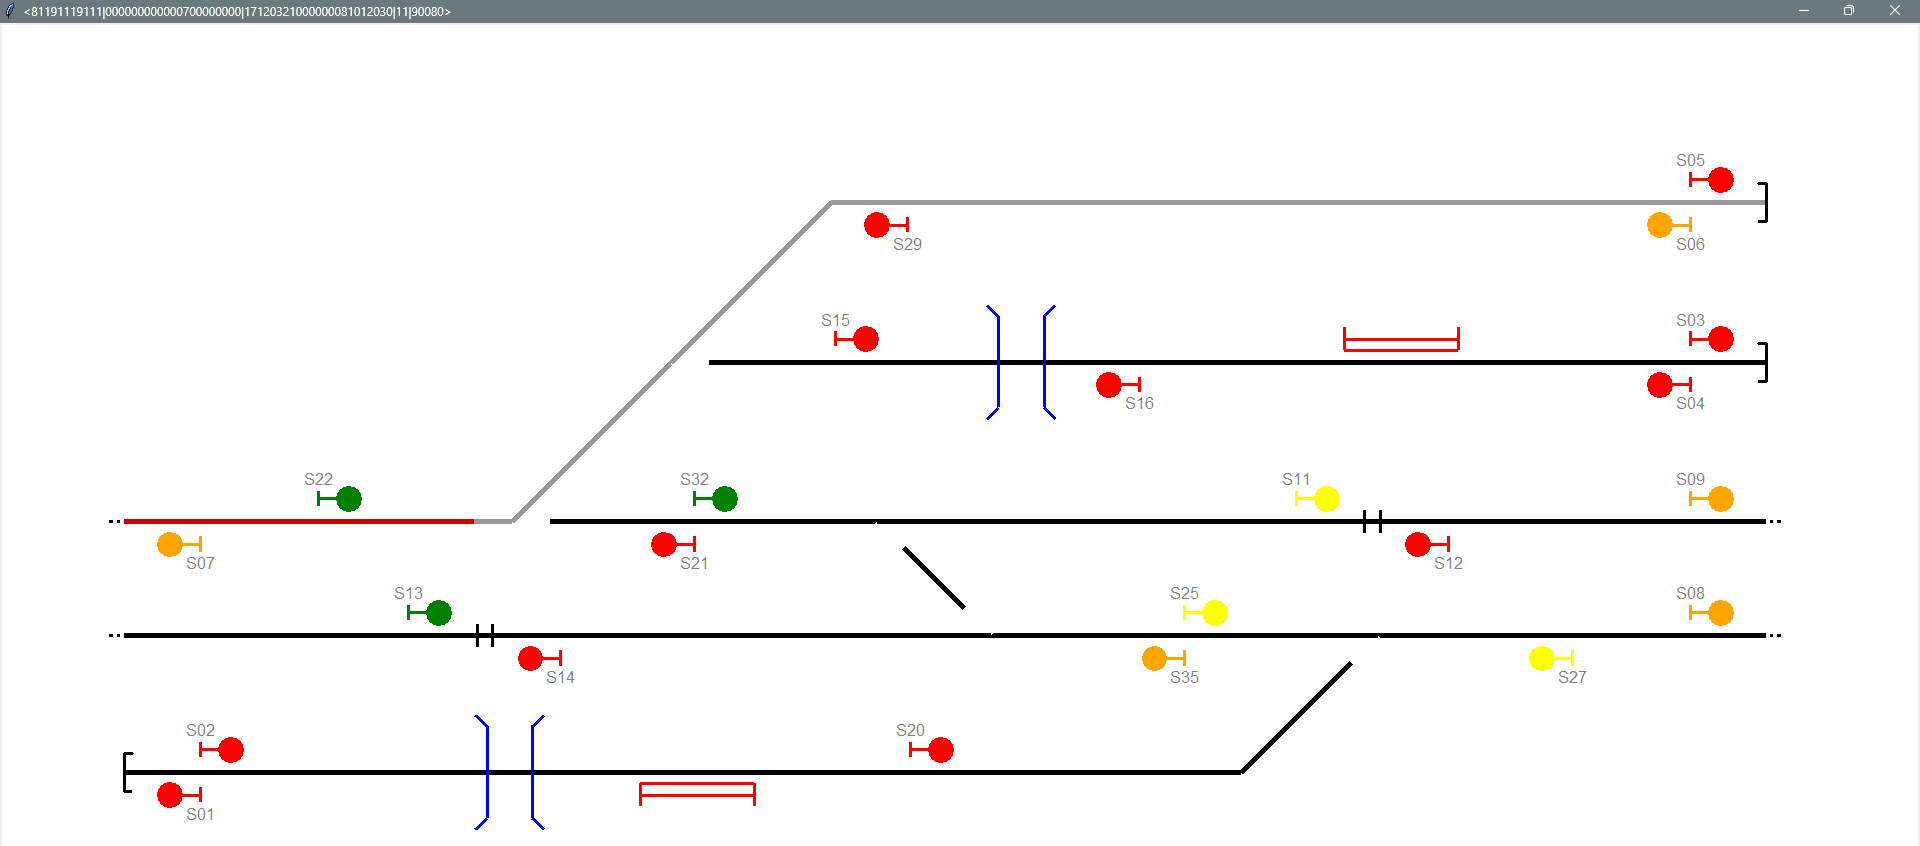
\includegraphics[origin = c, width=1\textwidth]{resultados-obtenidos/ejemplo1/images/AGG_R13}
		\centering\caption{Ruta 13 del ejemplo 1 en ejecución.}
		\label{fig:EJ1_AGG_R13}
	\end{figure}
	
	Continuando con el ejemplo referido a la R13, cualquier pedido de rutas que involucre en forma parcial o total elementos de la infraestructura que formen parte de la ruta que está seleccionada, que en este caso es R13, no será aceptada hasta que la misma sea liberada. La liberación puede darse por tres motivos: cancelación de la ruta (ver Sección \ref{sec:function_3}), timeout durante la comprobación del estado de la infraestructura (ver Sección \ref{sec:function_3}) o liberación secuencial (ver Sección \ref{sec:ACG_liberacion}).	
	
	La Figura \ref{fig:EJ1_AGG_R12}	ilustra el caso de solicitud y aprobación de la ruta R12, para lo cual el usuario seleccionó la señal S22 y luego la señal S15. Asumiendo que R12 es la única ruta activada, a diferencia del caso anterior, esta ruta solicita, además de secciones libres y cambios de vías sin enclavar, que el paso a nivel Lc08 se encuentre cerrado, aún cuando el paso a nivel se encuentra después de la señal S15 de finalización de ruta. Esto se debe a la protección por solape explicada en la Sección \ref{sec:function_4}.

	\begin{figure}[H]
		\centering
		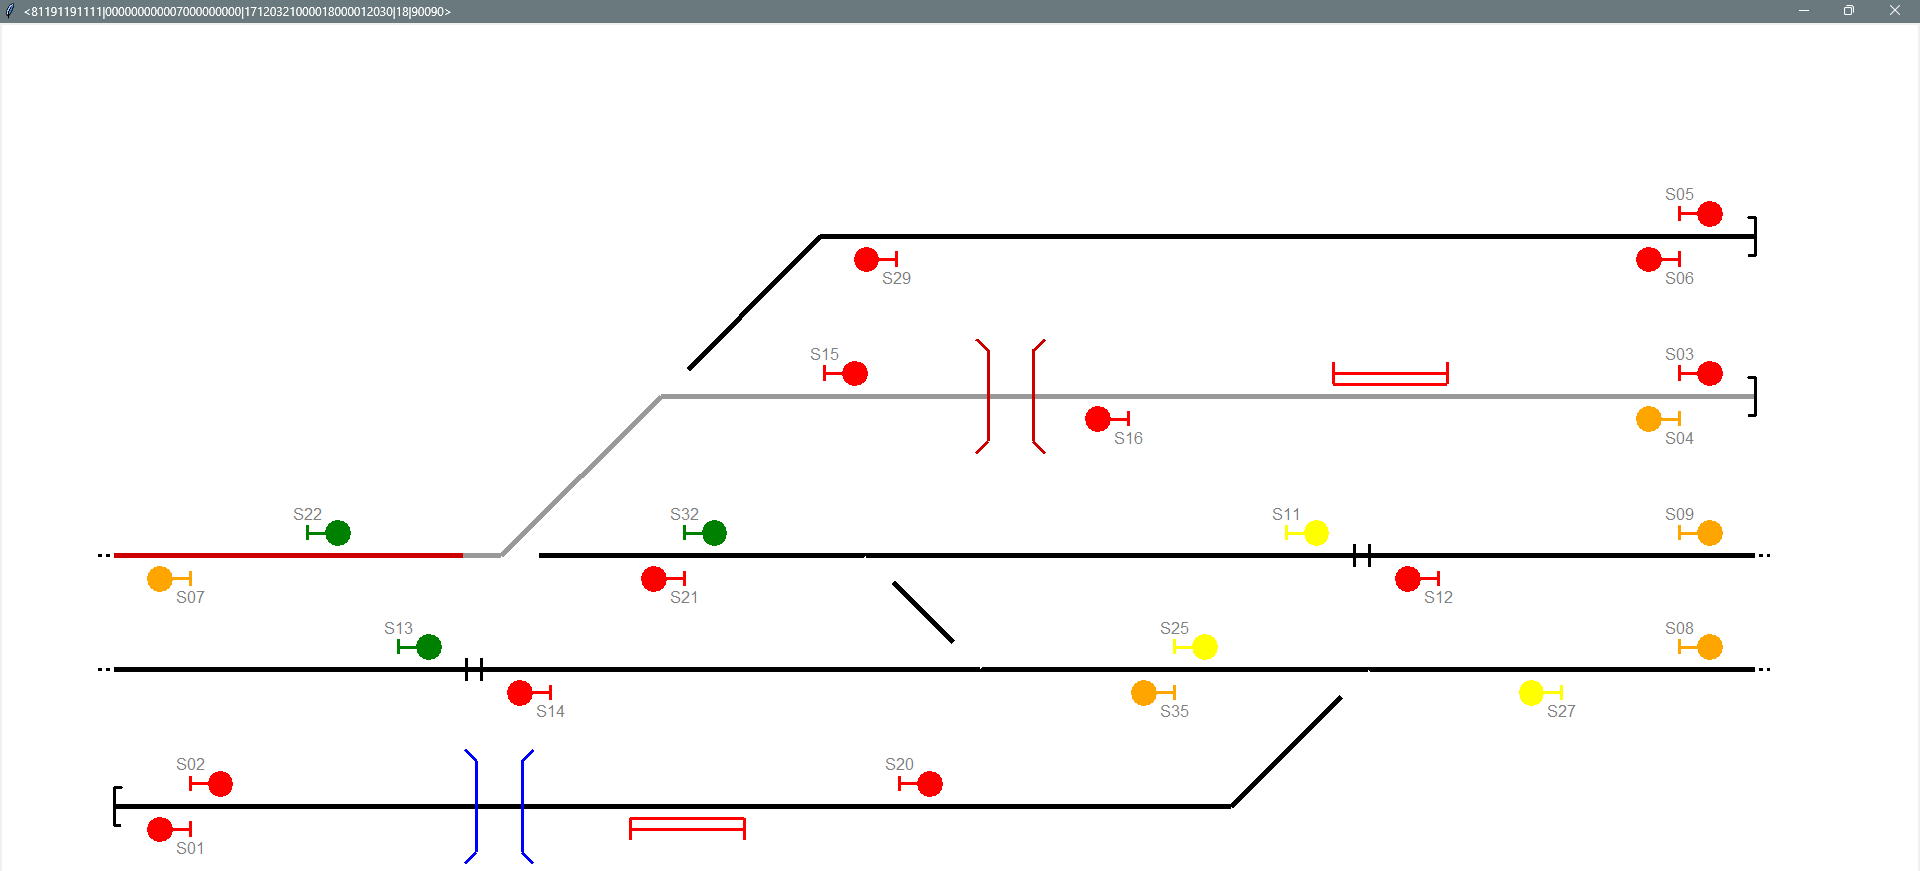
\includegraphics[origin = c, width=1\textwidth]{resultados-obtenidos/ejemplo1/images/AGG_R12}
		\centering\caption{Ruta 12 del ejemplo 1 en ejecución.}
		\label{fig:EJ1_AGG_R12}
	\end{figure}
	
	La Figura \ref{fig:EJ1_AGG_R19}	ilustra el caso de solicitud y aprobación de la ruta R19, para lo cual el usuario seleccionó la señal S32 y luego la señal S25. A diferencia de los otros casos expuestos, el sistema no sólo enclava los cambios de vías a utilizar (Sw12 y Sw13 en posición reversa), sino que también enclava el cambio de vías Sw06 en posición normal, debido a la protección por solape explicada en la Sección \ref{sec:function_4}.	
	
	\begin{figure}[H]
		\centering
		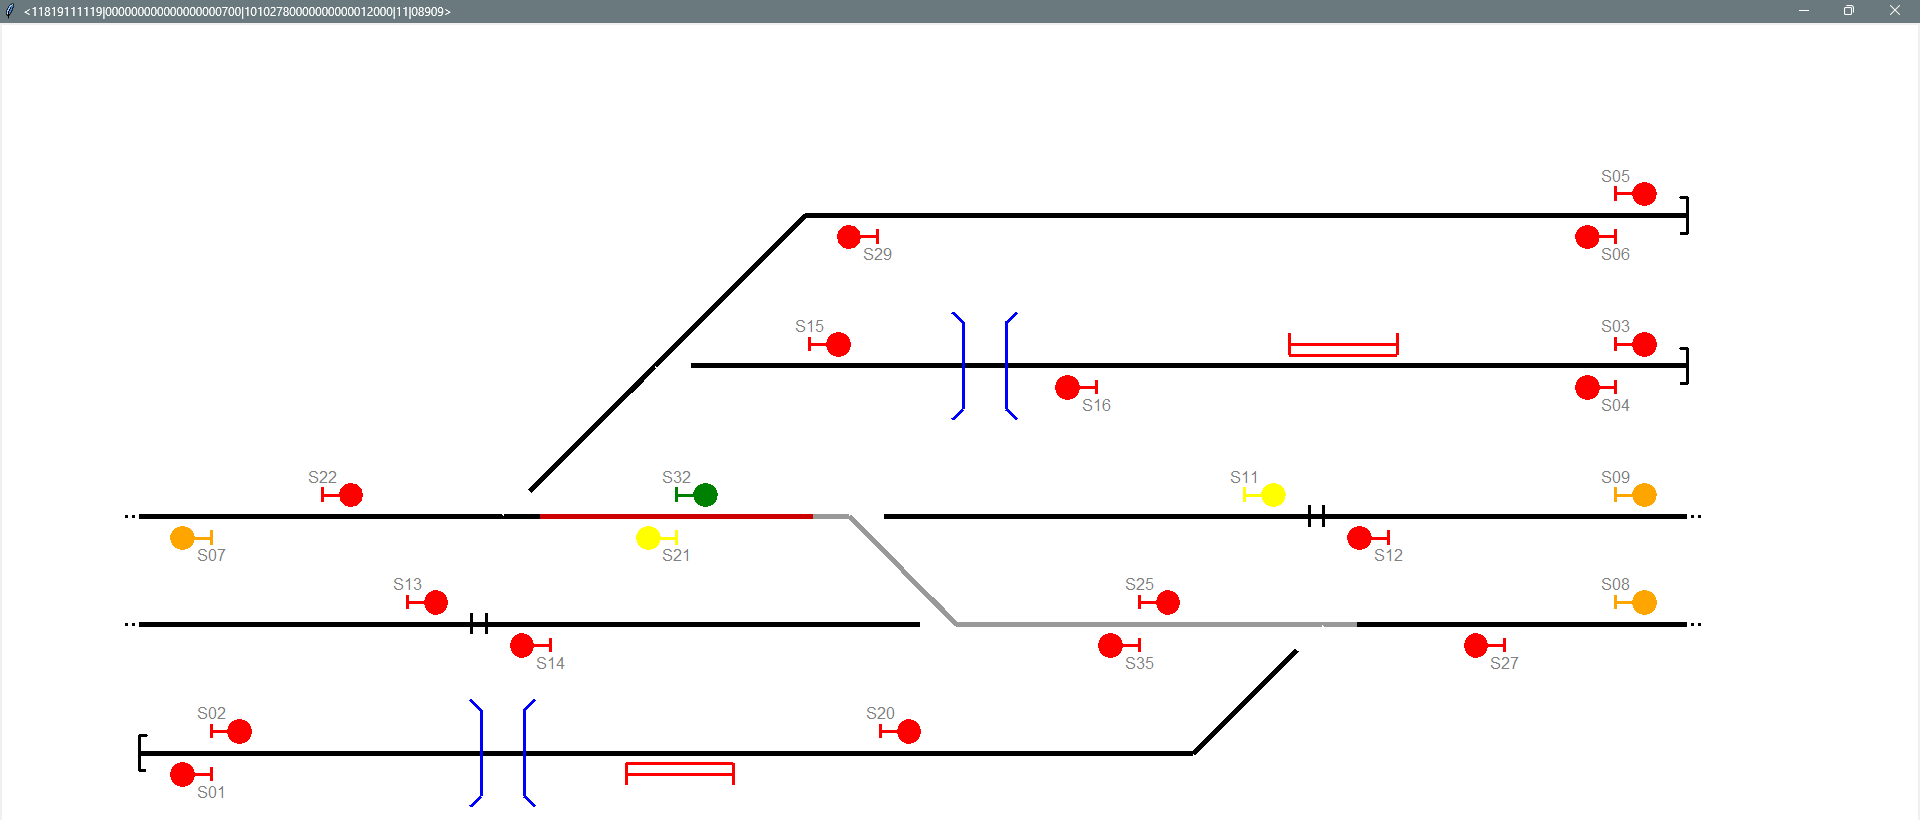
\includegraphics[origin = c, width=1\textwidth]{resultados-obtenidos/ejemplo1/images/AGG_R19}
		\centering\caption{Ruta 19 del ejemplo 1 en ejecución1.}
		\label{fig:EJ1_AGG_R19}
	\end{figure}
	
	Todas las rutas ilustradas en la tabla \ref{Tab:tabla_generated_1} fueron testeadas individualmente y en conjunto. La cancelación de rutas, timeouts y liberación secuencial fueron probadas con éxito pero al no ser posible de exponer en papel, fueron subidas en video, en un canal público para su visualización \cite{YOUTUBE}.	
	
	